\providecommand{\sid}[1]{\textbf{\texttt{#1}}}
\providecommand{\hzero}{\ensuremath{\mathrm{H}_{0}}\xspace}
\providecommand{\hzerostar}{\ensuremath{\mathrm{H}_{0}^{*}}\xspace}
\providecommand{\shrlm}{\textsc{SH-RLM}\xspace}
\providecommand{\TODO}[1]{\textcolor{red}{[TODO: #1]}}
\providecommand{\verdict}[1]{\textsf{#1}}

\section{Preliminary Optimization Runs}
\label{sec:diag}

\emph{These runs predate the study in Section~\ref{sec:setup}. They use a
different backbone (DeepSeek-V3.2) and a development branch with three extra
mechanisms that are not part of the study configuration. They exercised the
loop and informed its design. They are reported for transparency, not as the
paper's results.}

Validation tells the loop \emph{whether} an edit beat its incumbent, but not
\emph{why}. The per-length regression margins $\tau_\ell$ are also constants,
calibrated once on another backbone (DeepSeek-V4-Flash). We add three
mechanisms that address these gaps and test them in two runs with DeepSeek-V3.2
on AWS Bedrock (\$0.62/\$1.85 per million input/output tokens; cost is computed
from list prices).

\subsection{Method additions}

\paragraph{Advisory post-mortem.}
After each round, the validated candidate is replayed on up to six failed
\emph{held-in} instances from the pattern it targeted, plus up to three that the
incumbent passed. Each replay is paired with the incumbent's mining trace on the
same instance. The host first labels each instance \emph{improved},
\emph{regressed}, or \emph{within range}: F1 must leave the incumbent's attempt
range by more than $0.05$ to count as a change. A fixed model then assigns each
edit one verdict, \verdict{confirmed}, \verdict{refuted},
\verdict{not\_activated}, \verdict{inconclusive}, or
\verdict{regressed\_protected}, with trace citations and a one-sentence lesson.
The host rejects any verdict that contradicts its own facts, for example
\verdict{confirmed} with no improved target. Lessons go only to the next
proposer. The post-mortem never affects promotion and never reads held-out data.

\paragraph{Self-calibrated margins.}
Let $Q_\ell\in[0,1]^{n\times a}$ hold the incumbent's held-out F1 scores at
length $\ell$, for $n$ instances and $a$ attempts each. A nested bootstrap
simulates two evaluations of the same harness. It resamples instances with
replacement, then attempts within each instance:
\begin{equation}
  \hat{\Delta}_\ell =
  \Bigl|\tfrac{1}{na}\textstyle\sum_{i,j} Q_\ell[I^{A}_i,J^{A}_{ij}]
      - \tfrac{1}{na}\sum_{i,j} Q_\ell[I^{B}_i,J^{B}_{ij}]\Bigr|.
  \label{eq:boot}
\end{equation}
Each round sets $\tau_\ell=q_{0.95}(\hat{\Delta}_\ell)$, using 5000 replicates.
Only the regression margins change; the improvement threshold stays at
$\tau_{\mathrm{imp}}{=}0$.

\paragraph{Borderline re-test.}
Sometimes exactly one length misses its margin, by at most $\beta{=}0.03$, and
that miss alone blocks acceptance. Both harnesses then get $a$ more attempts at
that length only. The length is re-decided on the pooled $2a$ attempts, against
a margin from \cref{eq:boot} drawn at $2a$ attempts. A round runs at most one
re-test.

\subsection{Study 1: small-scale run}
The first run was small: 3 held-in and 3 held-out instances per length, one
attempt each, a 1200\,s limit per run, and frozen $\tau_\ell$. It ran two
rounds, and both were vetoed at 16K despite higher macro F1
(\cref{tab:smoke}). The post-mortem rated the round-1 \sid{S8} helper
\verdict{not\_activated}: \emph{``Adding a helper is insufficient if the root
doesn't invoke it.''} Round 2's proposer then suggested ``verify and
\emph{correct} misclassifications, not just report them.'' The run also exposed
the noise: mining the \emph{same} harness twice gave held-in macro F1 0.853 and
then 0.598. That noise motivated the calibration and the re-test. The run cost
about \$11.

\begin{table}[t]
\centering\small
\begin{tabular}{@{}lccccl@{}}
\toprule
 & 8K & 16K & 32K & Macro & Decision \\
\midrule
\hzero & .276 & .470 & .446 & .397 & -- \\
R1: \sid{S8} & .598 & .321 & .494 & .471 & 16K veto \\
R2: \sid{S4}+\sid{S6} & .561 & .280 & .491 & .444 & 16K veto \\
\bottomrule
\end{tabular}
\caption{Study 1: held-out F1 from 3 runs per length. The 16K margin was
0.144. Round 1's 16K delta was $-.149$ and round 2's was $-.191$.}
\label{tab:smoke}
\end{table}

\subsection{Study 2: full-size run}
This run recreates the screening-tournament setup at full size: 8 held-in and 8
held-out instances per length, 2 mining and 3 validation attempts, $k{=}4$
screened candidates, and patience 3. The earlier V4-Flash run of the same setup
recorded no promotion in three rounds.

None of round 1's 48 mining runs or 144 validation runs produced the exact gold
pair set. A pass-count gate could therefore never promote, and graded F1 is
necessary. Mining mostly found \texttt{mixed\_set\_error} failures. Screening
ranked four single-surface candidates. The winner, \sid{S4}, adds an
instruction to spot-check users near a predicate's threshold against their
original questions.

The calibrated margins were 0.143/0.158/0.252, close to the frozen
0.144/0.144/0.244. The candidate
improved F1 at every length and was promoted (\cref{tab:val}). It also costs
$1.51\times$ more per run, because it makes more sub-calls. The post-mortem
nonetheless returned \verdict{refuted}. Of six failed held-in instances, two
improved and four did not move. Its lesson: \emph{``verification that only logs
findings without corrective feedback loops cannot fix classification
errors.''}

Round 2 mined 48 fresh runs on the round-1 harness. Two reached the exact gold
pair set, both on the same instance. All four first-pass candidates failed
screening, with macro deltas from $-0.111$ to $-0.222$. The loop then
re-attributed the same mining runs, with no new rollouts, and proposed again.
Two of the four new candidates passed screening. The top-ranked one, again
\sid{S4}, tells the model to reclassify a question and recompute the user sets
when it finds a mismatch, the corrective step that round 1's lesson found
missing.

The recalibrated margins were 0.150/0.129/0.173, so the 32K margin fell from
0.252 to 0.173 between rounds on the same model. The macro gain shrank from
+0.054 in screening to +0.013 in full validation (\cref{tab:val}). No length
crossed its margin, so no re-test ran, and cost per run was unchanged
($0.99\times$). The candidate was promoted, although none of the 144 validation
runs in this round produced the exact gold set. The post-mortem again returned
\verdict{refuted}. All three target instances stayed within the incumbent's
range, and the one protected instance fell from F1 1.0 to 0.934, which the
post-mortem attributes to a correct question being reclassified. Its lesson:
\emph{``Cross-checking classifications alone is insufficient.''} We stopped the
run after this round to keep budget for the long-context test, so no proposer
has used this lesson. The two rounds cost about \$94 in completed runs and
attribution, proposal and post-mortem calls.

\begin{table}[t]
\centering\small
\setlength{\tabcolsep}{7pt}
\renewcommand{\arraystretch}{1.2}
\begin{tabular}{@{}lcccc@{}}
\toprule
 & 8K & 16K & 32K & Macro \\
\midrule
\hzero & .700 & .746 & .609 & .685 \\
R1: \sid{S4}$^\dagger$ & .740 & .765 & .719 & .741 \\
\addlinespace
$\Delta$ & +.039 & +.019 & +.110 & +.056 \\
Veto line & $-$.143 & $-$.158 & $-$.252 & -- \\
\midrule
R2: \sid{S4}$^\dagger$ & .752 & .736 & .775 & .754 \\
\addlinespace
$\Delta$ & +.012 & $-$.029 & +.056 & +.013 \\
Veto line & $-$.150 & $-$.129 & $-$.173 & -- \\
\bottomrule
\end{tabular}
\caption{Study 2: held-out F1 from 24 runs per length (8 instances $\times$ 3
attempts). $^\dagger$Promoted. Each $\Delta$ is against that round's incumbent:
\hzero in round 1 and the R1 harness in round 2, whose validation runs were
reused. The veto lines are each round's self-calibrated margins.}
\label{tab:val}
\end{table}

\paragraph{Long-context test.}
We compare the frozen \shrlm harness with \hzerostar on the 256K OOLONG-Pairs
test set, which is 8$\times$ the longest optimization length. All four
conditions run on the same 9 tasks (3 per task group) with 3 attempts each, and all 9 ran
to completion (\cref{tab:long}). \shrlm scores higher on every task. Most of
the gap comes from how \hzerostar fails: 9 of its 27 runs end in
\texttt{wrong\_format} and score 0, and its runs average 592\,s, against
4094\,s for \shrlm. So \hzerostar mostly answers without classifying the
256K context question by question. \shrlm does that work, and its promoted
spot-check and reclassify steps still apply at this length. It costs
$1.5\times$ more per run.

Against the other two conditions the picture is weaker. \shrlm and \hzero are
tied: the difference is +.048, with a CI that includes 0, and \shrlm wins 6 of 9
tasks. \hzero also classifies question by question (4463\,s per run), but 2 of
its runs end in \texttt{wrong\_format} and 2 more are terminated. Most of
\shrlm's gain over \hzerostar therefore reflects \hzerostar's failures, not an
improvement over \hzero. $\lambda$-RLM is the strongest condition. It beats
\shrlm by .135 (CI excludes 0) and wins all 9 tasks, at $0.14\times$ the cost
per run and about 110\,s per run.
\Cref{fig:long} places the four conditions on quality and cost. $\lambda$-RLM is both the
most accurate and the cheapest condition, so it dominates the other three. \shrlm and
\hzero sit close together at the expensive end, and only the difference
against \hzerostar has a confidence interval clear of 0 in \shrlm's favor.

\begin{figure}[t]
\centering
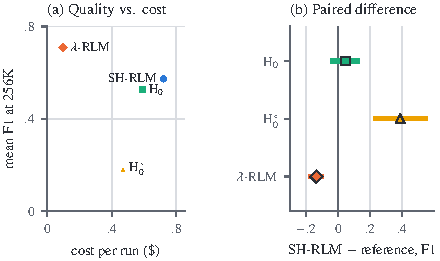
\includegraphics[width=\linewidth]{aaai27/figures/fig_long_context.pdf}
\caption{256K OOLONG-Pairs test (DeepSeek-V3.2; 9 tasks $\times$ 3
attempts per condition). (a)~Mean F1 against mean cost per run.
(b)~\shrlm minus each reference with task-level paired bootstrap 95\%
intervals; right of 0 favors \shrlm. Data as in \Cref{tab:long}.}
\label{fig:long}
\end{figure}

\begin{table}[t]
\centering\small
\begin{tabular}{@{}lccc@{}}
\toprule
256K & Tasks & Mean F1 & Cost/run \\
\midrule
\hzero & 9 & .526 & \$0.59 \\
\hzerostar & 9 & .185 & \$0.47 \\
$\lambda$-RLM & 9 & .708 & \$0.10 \\
\shrlm & 9 & .573 & \$0.72 \\
\bottomrule
\end{tabular}
\caption{Long-context generalization on matched tasks: 9 tasks $\times$ 3
attempts per condition, all complete. Paired difference +.388, 95\% bootstrap CI
[+.220, +.556]; \shrlm wins all 9 tasks. Against \hzero: +.048
[$-$.045, +.134]. Against $\lambda$-RLM: $-$.135 [$-$.187, $-$.088].}
\label{tab:long}
\end{table}

\paragraph{Discussion and limitations.}
The round-1 gain (+0.056) is below the bootstrap's noise level for macro F1
(0.108). Under $\tau_{\mathrm{imp}}{=}0$, the promotion is therefore a
selection decision, not a significant improvement. Round 2's gain (+0.013) is
further below its noise level (0.088), so its promotion is at most a tie-break
over the round-1 harness. That comparison also reuses the validation runs on
which the round-1 harness was selected, which may flatter the incumbent. The
post-mortems also suggest that neither edit worked through its stated
mechanism. The 256K test, the first independent check, does not show a gain over
\hzero, and $\lambda$-RLM outperforms both at a fraction of the cost. The 256K
set has only 9 tasks from two context windows. The bootstrap resamples instances
independently for the two harnesses, but validation compares them on the same
instances. The margins therefore overstate the noise, and a paired version
would tighten them. Each study is a single trajectory, with no run that
disables the post-mortem, so its benefit is not yet measured. Held-out sets are
small: 8 instances per length, drawn from two record collections. The code is
on branch \texttt{ELIAZ-LAST-SHOT} (commits \texttt{960fb7c6},
\texttt{2700c628}, \texttt{c1e3353b}; post-mortem first added in
\texttt{b961b4ce}).
